\documentclass{ctexart}
\usepackage{graphicx}
\usepackage{hyperref}
\usepackage{booktabs}
\title{文献综述与选题书面报告 \\ \normalsize{论文题目:基于信息论度量的社群发现理论与算法研究 }
}
\author{赵丰 \\ 学号: 2017310711}
\begin{document}
\maketitle
\section{选题背景及其意义}
在网络科学中,复杂的网络结构往往存在一定的社群结构 \cite{fortunato2010community} 。社群结构是指
具有相同特征的节点集合,
比如社交网络中的圈子、流行病网络中集中爆发的区域。以及在自然界中的群落以及微观世界网络中的大分子
蛋白质。社群发现是通过一定的方法寻找网络中特定的社群结构。在自然科学研究中有助于发现特定的结构。而在
技术领域则是实现某项技术目标的重要一环。比如在分布式计算中划分子任务使得不同的子任务之间有尽可能
小的耦合,在推荐系统设计中划分用户社群以实现精准推荐。社群发现的实现离不开特定的算法,而好的社群发现算法
需要有特定的理论支撑,以便助其在各领域实现广泛应用。

社群发现算法需要适合特定的场景。考虑到有一些问题中社群之间具有复杂的相关关系,从而构成一定的层次结构。如
在社交网络中根据兴趣对目标人群的划分则有大的尺度和精细的尺度多个维度。普通的社群发现算法无法适应社群的层次
结构划分的需要。基于特定理论的指导,研究新的分层发现算法对解决某些特定应用场景的问题具有重要的实用价值。

社群发现有大量的算法可供使用。由于对社群发现问题的概率模型的理论
极限和部分经典算法的信息学含义缺少足够的认识,这些启发式算法在消耗大量计算资源的同时效果也
不一定能得到保障。为解决该问题,需要对社群发现的理论模型开展深入研究。
社群发现理论的研究是一个涉及信息论、图论和概率论等多学科交叉融合的领域。目前基于随机块模型的理论研究思路
取得了一定的突破,随机块模型提供了比较不同的社群发现算法的标准化人工生成的数据集。此外,从理论层面研究随机块模型下算法的误差可以
指导算法的设计。
目前的研究给出了若干
在随机块模型下具有理论保证的几类算法,通过对这些算法做出近似和调整,可以适用于实际的社群发现问题。随机块模型的研究
还可以用于解决和社群发现密切相关的问题,比如根据若干次民意调查的结果预测选民的政治倾向等。

在分析具有图结构的数据时,通常每个节点会有一些额外的信息可供使用,比如每个节点的特征属性。比如在社交网络中利用
用户间的交互关系和每一用户自身的属性对用户群体进行划分。在生物信息学中利用
基因本身的信息和不同基因之间的互信息对基因进行聚类 \cite{4359897}。

如何利用这些节点的观测值提高
社群发现的准确率也是近年来研究的一个热点。已经涌现了大量的算法可以利用节点和图的信息进行社群发现,但在这方面缺少
针对误差速率的理论分析。这方面的理论分析可以指导特征数量的选取,以提高数据的使用效率,避免浪费。此外,这一部分的研究
还可以用在其他具有相似数学模型的领域。比如有相关关系的多个数据源的信息压缩问题。

信息论的度量如熵、互信息等最初是在通信领域用于度量编码和信道传输的理论极限,逐渐被
推广到了机器学习、网络科学等领域。信息论的度量如 KL 散度、互信息等 可以作为算法的评价指标,
以及出现在理论模型中误差的理论极限中。利用信息论中误差指数的研究方法,可以有效地分析最大似然算法在随机块模型上的
恢复误差。


\section{国内外研究动态}
社群发现问题的研究和机器学习的聚类问题有共通之处。即都是将数据划分出一定的层次结构。不同之处在于数据的形式不同,
聚类中考虑的是每个数据都有一个特征向量,而社群发现是针对图的数据结构。这两类结构之间是可以相互转换的,比如通过
k近邻的方法可以从数据特征构造表征数据间相似程度的图。反之,通过特征嵌入 (feature embedding) 的技术由图可以
获取每个节点的数据特征 \cite{hamilton2017representation}。通过这样的相互转换,聚类算法和社群发现算法可以通用。但由于这种转换会损失掉一部分原始信息
并且具有一定的计算复杂度,通常意义上的聚类算法直接针对数据特征进行处理而社群发现是针对图进行处理。通过使用图的结构对网络
进行数学建模,社群即是图的子图。

社群发现领域的研究根据研究层面可大致划分为理论研究、算法设计与分析以及应用研究三个层面。
理论研究主要是基于某种统计模型生成随机图进行研究,常用的统计模型有贝叶斯模型和随机块模型 (Stochastic Block Model)。
算法设计主要分为两类算法,一类是启发式算法,比如通过去除图的边和聚合图中的点获取社群。还有一类是指标优化式算法,
即通过求解某一优化问题获得社群结构,比如最小化各社群之间边的权值之和,或者求解模块度的最大值 \cite{newman2006modularity}。
而应用层面的研究主要集中在生物网络和社交网络方面,通常需要和特征提取等工程步骤结合起来才能实现一次比较有意义的数据挖掘工作。

如同选题背景中所介绍的,本课题主要包含层次发现算法、随机块模型的精确恢复问题及有额外信息的随机块模型三个方面。
下面将从这三个方面分别阐述国内外研究的动态。
\subsection{层次发现算法}

最早的层次发现算法是系统聚类法 \cite{slink},即根据欧式度量每次聚合两个节点形成聚类树。
近年来基于各领域的学科知识出现了大量新的聚类算法,比如
贝叶斯聚类方法 \cite{bhc}、基于图论和离散数学的方法 \cite{dasgupta2016cost}
。
这些方法在模型复杂性,效率和准确性方面有着不同的权衡。
例如,有一种拓展了贝叶斯聚类的方法 \cite{blundell2011discovering}
在给定的概率模型下
可以产生非二叉结构的层次树。贝叶斯聚类的方法考虑了数据的分布,不能直接用于社群发现的场景。有学者将其进行改造,提出了
贝叶斯社群发现的算法\cite{RN23},在某些数据集上有较好的表现。
贝叶斯模型总体说来有许多超参数需要调整,其层次发现结果可能因其固有的随机性而有很大差异。 因此,在实际应用中,不适合使用基于贝叶斯的模型来解决具有稳定需求的问题。 

除了上面提到的分层发现方法外,有学者利用信息论度量研究聚类问题。他们的出发点是基于以下观察结果:层次聚类中的指标
这些数据主要是根据经验得出的,可能无法反映出数据真实的概率模型。
在过去的文献中,使用了其他某种信息理论量度 \cite{ic2002} 或互信息\cite{mim}。
这些现有研究存在一些缺点。首先,信息度量是使用 Parzen 窗口根据数据进行估计的,该窗口是一种高斯混合模型。对于这种参数化方法,如果数据真实的分布与假设相距甚远,则结果会很不准确。
其次,只有贪心算法才能逼近基于信息论的损失函数的最小值。 
直到有学者提出群集中的多元互信息度量标准后,在这一方面才有所突破 \cite{ic2016}。 

该多变量互信息的度量可以处理对随机变量进行聚类的问题,在两两独立的网络模型 \cite{pin}
中其数学结构与最小平均分割一致  \cite{mac}。最小平均分割,也叫图强度 \cite{cunningham1985optimal},是在不给定分割数的情况下求解
平均最小割问题。与最小割是NP难不同的是,最小平均分割可以在多项式时间内求解。第一个算法由 Narayanan 提出,利用了主分格序列这样一种结构 \cite{narayanan}。后面有人通过参数化最大流的方式加以改进 \cite{RN17}。但该方法利用了某种并行化的方法,以及受到数值精度的影响,虽然在理论分析中复杂度
比 \cite{narayanan} 快一个数量级,但在实际算法中难以实现。

异常值检测问题 \cite{grubbs1969procedures} 和聚类分析有着密切的联系,利用基于诸如局部异常因子 \cite{Breunig} 等方法需要提前知道异常值点的数量、以及需要设置一些超参数的值。
\subsection{随机块模型的精确恢复问题}
随机块模型被用在了度量不同的社群发现算法的基准数据集,也叫 种植 k-分区模型,其中 k 是社群的数量 。
随机块模型的生成是先给定 n 个节点,再根据节点所属的类别随机地生成边。同类节点之间有边相连的概率(记为 p)大,而
不同类节点之间有边相连的概率(记为 q)小。\cite{abbe2017community}

在已知每个节点真实标签的情况下,衡量算法在随机块模型的恢复性能通常
使用错误率的方式,即考虑在何种条件下,随着图的规模 n 趋向于无穷,错误率趋向于零。
最常用的错误率是恢复错的节点的比例,基于此种错误率的理论研究我们称之为弱恢复(weak recovery)。
与之相对应的强恢复 (strong recovery) 是考虑全部节点不出错的情况。

在弱恢复的研究中,通常是考虑 p, q 在 $\frac{1}{n}$ 这一数量级,因为对于更稀疏的图,无法实现弱恢复的目标。
对于两类的随机块模型并且 $p=\frac{a}{n}, q = \frac{b}{n}$。2014年前后证明了弱恢复的充要条件是 $(a-b)^2 > 2(a+b)$
\cite{mossel2015reconstruction, mossel2018proof}。

在强恢复的研究中,通常是考虑 p, q 在 $\frac{\log}{n}$ 这一数量级,因为对于更稀疏的图,无法实现强恢复的目标。
对于两类的随机块模型并且 $p=\frac{a \log n}{n}, q = \frac{b \log n }{n}$。2015年前后证明了强恢复的充要条件是
$\sqrt{a} - \sqrt{b} > \sqrt{2}$ \cite{abbe2015exact, mossel2016}。这个结果随后推广到了 k 个
社群以及更一般的随机块模型中\cite{abbe2015community}。

Ising 模型是一种刻划节点状态的概率模型 \cite{ising1925beitrag},最早提出的时候是两状态的。但可以推广至多状态的 Ising 模型 \cite{potts1952some}。
同时考虑 Ising 模型 和 SBM 模型的研究,最早有学者研究了如何计算定义在SBM模型生成的图上的Ising 模型的配分函数 \cite{liu2017log}。
后来又有学者研究 了定义在静态图上的 Ising 模型的相变问题 \cite{berthet2019exact} 以及样本复杂度问题等 \cite{ye2020exact}。
关于该样本复杂度的问题一个应用背景是在用多次民意调查估计选民的政治倾向中所需的调查次数。

在 SBM 和 Ising 复合模型的样本复杂度研究中,SBM 精确恢复的充要条件可以作为一个特例得到 \cite{ye2020exact}。
因此该复合模型可看作随机块模型的一个拓展。类似得还有很多其他思路的拓展也可以导出此充要条件,如 互测量 \cite{chen2016information}、 最小最大速率 \cite{zhang2016} 等。

关于 SBM 模型算法错误率的一个误差上界在推导强恢复的充分条件时给出 \cite{abbe2015exact},但有提升空间。
此外,关于最大似然算法和最大模块度算法的联系之间已有学者进行了研究 \cite{newman2016equivalence}。
最大模块度算法的优化目标是 NP 难的,最早使用贪心法近似求解 \cite{clauset2004finding},后来有学者使用模拟退火的方法近似求解 \cite{he2016fast}。除了最大模块度算法外,在基于2个社群的SBM生成模型的社群发现算法设计与分析中,还有学者基于半正定规划 \cite{hajek2016achieving}、谱分解\cite{abbe2020entrywise}(求解随机邻接矩阵的第二特征向量)、非凸优化的方法求解 SBM的社群发现问题\cite{wang2021non}。这些工作的难点在于分析算法可以在强恢复的条件下可以实现
精确恢复。
模拟退火的方法和 梅特罗波利斯 (Metropolis) 采样算法原理一样,只是表述不同,后者常用于 Ising 模型的采样 \cite{metropolis1953equation}。

关于 SBM 的参数估计问题也有相关的研究工作。在弱恢复的场景下 Mossel 提出了参数 $(a,b)$ 的一个一致估计量
\cite{mossel2015reconstruction}。对于比弱恢复更稠密的情形,通常可以先恢复节点的标签,再估计模型参数
\cite{abbe2015recovering}。

\subsection{有额外信息的随机块模型}
通常添加额外信息外,基于随机块模型的社群发现能达到更高的准确率。通常额外信息具有多种形式,
比如部分已知正常标签的节点、全部节点的标签通过一个 BSC 的有噪信道以及根据节点的标签基于不同的分布生成一些观测值\cite{saad2018community}。
这一部分的研究工作可以应用在社交网络分析中,比如利用用户间的交互关系与
每一用户自身的属性对用户群体进行划分。

已知正常标签的节点、全部节点的标签通过一个 BSC 的有噪信道两种情形,已经有学者在SBM精确恢复的框架下
研究出了它们可恢复的充要条件和可实现精确恢复的半正定规划算法 \cite{esmaeili2019community, esmaeili2019exact}。
用 尖峰协方差模型 (spiked covariance model) 对额外信息
进行建模,
有学者研究了两社群弱恢复的充要条件 \cite{deshpande2018contextual}。
% one result comes from 2021 ISIT submitted paper
而对于根据节点的标签基于不同的分布生成一些观测值的场景,对于一般的情形,有学者在
研究图上的数据压缩问题时顺带给出了一个精确恢复的充要条件 \cite{abbe17sideinfo}。

SBM 问题的精确恢复条件本身蕴含着某种对称性,相应的可以用 Rényi 散度来刻划。这一个结论实际是对于具有
对称分布的一般假设检测问题的特例 \cite{gao2018community}。

利用半正定规划算法实现 SBM 的精确恢复,在多种假设下都可以达到最优条件 \cite{hajek2016achieving},是最大似然算法好的近似 。在算法设计层面,利用 对称的 SBM 的结构,基于 ADMM 的迭代策略,有学者提出了 SDP-1的算法 \cite{amini2018semidefinite}。
\section{课题研究内容}
本课题研究的内容主要可分为以下三方面, 这三方面的内容是有一定内在联系的
的。
\subsection{层次发现算法}
基于最小平均分割,研究社群发现
的层次发现算法是本工作的一个研究内容。这一部分的研究又可分为理论性质讨论、算法设计研究和算法应用研究三个小部分。
在理论性质讨论部分,重点研究的是在何种条件下最小平均分割给出非平凡的解以及其他的等价定义等。
在算法设计研究部分,重点研究的是从算法结构层面改进已有的算法,降低算法的复杂度。
在算法应用研究层面,重点考虑该方法在异常值检测中的应用。
\subsection{随机块模型的精确恢复问题}
前一部分的研究中涉及图中的分割的概念,利用分割定义能量函数、进而构造图上的 Ising 模型并利用
Ising 模型研究随机块的精确恢复问题是本部分的研究重点。这一部分的研究起到承上启下的作用,一方面
它发展了前一部分研究的最小分割的方法,
另一方面
它提出的理论研究方法和半正定规划的算法实现可以应用到后续的有额外信息的随机块模型的研究中。
\subsection{有额外信息的随机块模型}
在前两部分的研究基础上,该部分的研究将考虑有额外信息的随机块模型。通过错误概率的形式定量的刻划额外信息
对随机块模型精确恢复的贡献。此外,本部分的另一个研究重点是设计半正定规划算法实现
有额外信息的随机块模型的精确恢复,给出了一个可以用计算机算法实现的形式。
\section{研究方案}
这里我将基于已有的研究成果, 简要介绍我下一步的研究方案。
\subsection{层次发现算法}
我们研究了图上的最小平均分割的理论性质,并基于此设计了社群的层次发现算法。该算法
不需指定分割数量即可自动划分图的层次结构。在算法的实现层面,在分治的
思想指导下,我们利用子图与图的关系,改进了已有的算法,使得算法的
时间复杂度降低了一个数量级。最后,我们还将层次发现算法应用在了异常值检测领域,
提出了检测边界方程的概念,在一些具有较复杂的分布情形下有良好的检测效果。


\subsection{随机块模型的精确恢复问题}
\begin{figure}
	\centering
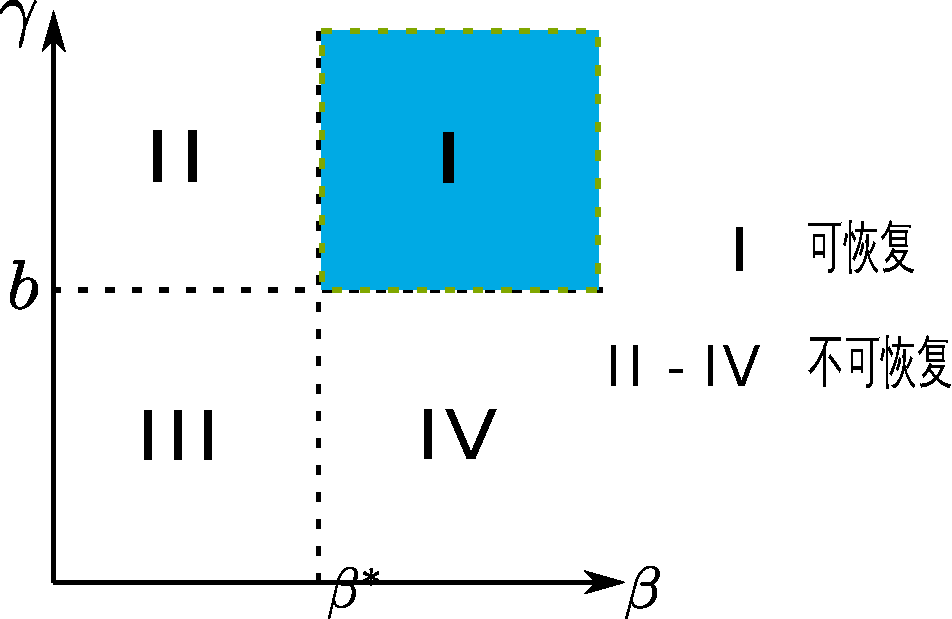
\includegraphics[width=6cm]{phase_trans.pdf}
\caption{Ising 模型精确恢复的充要条件(相变现象)}\label{fig}
\end{figure}
基于定义在随机块上的 Ising 模型,我们研究了利用该模型随机产生一个样本做精确恢复的误差。
该模型的参数由 $(\beta, \gamma)$ 组成,如图 \ref{fig} 所示, 只有在 $\beta > \beta^*$ 且 $\gamma > b$的条件
下才能实现精确恢复。除此之外,我们还从最小化Ising 模型的能量的角度研究了精确恢复的误差上界。这一小部分的研究
又可分有无约束优化和有约束优化两种陈述。通过这一部分研究,我们建立了最大似然算法、最大模块度算法、最小割算法和 Ising 模型
的联系。最后,我们基于梅特罗波利斯采样算法给出了Ising 模型的算法可实现的形式。并用该算法对相变现象
进行了实验验证。下一步将重点研究相变点 $\beta = \beta^*$ 处的精确恢复误差以及考虑
用多个 Ising 模型的采样做精确恢复的相变条件。

\subsection{有额外信息的随机块模型}
在这一部分的研究中,我们从假设检测中的误差指数和随机块模型
精确恢复的已有结果入手,研究了有额外信息的随机块模型的精确恢复的误差。我们考虑的模型是
各社群节点数量均相等 的 SBM 模型。此外,我们设计了半正定规划算法,在误差指数大于零的条件下,可实现有额外信息的随机块模型的精确恢复。
下一步我们将重点研究该模型的相变条件。

\section{工作特色及难点}
本课题的特点是利用信息论的度量,在相关理论的指导下研究社群发现的理论极限和算法设计。
如何把理论分析和实际应用的算法结合起来,是本工作的难点。为了克服该难点,
在“理论-算法-应用”三者衔接的时候需要引入一些假设并对问题做出
化简, 排除次要因素, 以提炼出问题的本质。
\section{预期成果和可能的创新点}
以上工作已发表一篇期刊论文和1篇会议论文,预期在第三部分工作上发表1篇会议论文。

本工作的主要创新点体现在如下三个方面:
\begin{enumerate}
\item \textbf{基于最小平均分割的层次发现}:
研究基于最小平均分割的层次发现算法的理论性质;
改进已有的层次发现算法,时间复杂度降低一个数量级。
\item \textbf{随机块模型的精确恢复问题研究}:
研究基于 Ising 模型的算法精确恢复条件与误差衰减速率;
揭示与其他社群发现算法的关系。
\item \textbf{有额外信息的随机块模型}:
推导融合模型错误率的理论极限;
针对融合模型设计半正定规划算法,可实现精确恢复。
\end{enumerate}
\section{论文工作的总体安排}
论文工作的总体安排如表 \ref{tab} 所示。
\begin{table}[!ht]
		\centering
	\begin{tabular}{cc}
		\toprule
		时间 & 研究内容 \\
		\hline
		2021年4月-2021年7月 & 进一步研究有额外信息的随机块模型\\
		2021年8月-2021年12月 & 进一步研究随机块模型的精确恢复问题\\
		2022年1月-2022年6月 & 整理资料、撰写博士论文\\
		\toprule		
	\end{tabular}
	\caption{论文工作的总体安排}\label{tab}
	\end{table}
\bibliographystyle{unsrt}
\bibliography{exportlist.bib}
\end{document}
